%%%%%%%%%%%%%%%%%%%%%%%%%%%%%%%%%%%%%%%%%%%%%%%%%%%%%%%%%%%%%%%%%%%%%%
% writeLaTeX Example: Academic Paper Template
%
% Source: http://www.writelatex.com
% 
% Feel free to distribute this example, but please keep the referral
% to writelatex.com
% 
%%%%%%%%%%%%%%%%%%%%%%%%%%%%%%%%%%%%%%%%%%%%%%%%%%%%%%%%%%%%%%%%%%%%%%
% How to use writeLaTeX: 
%
% You edit the source code here on the left, and the preview on the
% right shows you the result within a few seconds.
%
% Bookmark this page and share the URL with your co-authors. They can
% edit at the same time!
%
% You can upload figures, bibliographies, custom classes and
% styles using the files menu.
%
% If you're new to LaTeX, the wikibook is a great place to start:
% http://en.wikibooks.org/wiki/LaTeX
%
%%%%%%%%%%%%%%%%%%%%%%%%%%%%%%%%%%%%%%%%%%%%%%%%%%%%%%%%%%%%%%%%%%%%%%
\documentclass[twocolumn,showpacs,%
  nofootinbib,aps,superscriptaddress,%
  eqsecnum,prd,notitlepage,showkeys,10pt]{revtex4-1}
  
\usepackage{graphicx}
\graphicspath{ {images/} }

\usepackage{amssymb}
\usepackage{amsmath}
\usepackage{graphicx}
\usepackage{dcolumn}
\usepackage{hyperref}

\begin{document}

\title{Formally proving equivalence between abstract and concrete specifications of HMAC}
\author{Katherine Ye, advised by Andrew Appel}
\affiliation{Princeton University}

\begin{abstract}
The OpenSSL implementation of HMAC has been proven to correctly implement its concrete specification. HMAC uses SHA-256 as its hash function, and the SHA-256 program has also been proven to correctly implement its specification. At a higher level, HMAC has been proven "safe to use": an abstract specification of HMAC has been proven to be a pseudo-random function given that its internal hash function is one as well. We bridge the gap between the abstract and the concrete HMAC spec by formally proving their equivalence. This proof transfers the desirable and necessary property of being a pseudo-random function (with some caveats) to both the concrete spec and the C implementation of HMAC, guaranteeing that the OpenSSL code is "safe to use."
\\
TODO shorten abstract (December 26, 2014)

\end{abstract}

\maketitle

\section{Introduction}

Compelling quote or hook here TODO

There exists a gap between mathematical cryptography (rigorous paper proofs of correctness of an algorithm) and applied cryptography (concrete implementations of those algorithms, plus the field of information security). This gap gives us two reasons to be wary. First, the paper proofs may be flawed, leading us to believe that algorithms are "safe to use" when they are not. (TODO example of wrong crypto proof) Second, even if the proofs are right, they are accompanied by a specification of the algorithm only on paper. The concrete code implementing this specification may contain exploitable bugs, allowing hackers to induce buffer overflows, ... TODO (TODO OpenSSL, Heartbleed) 

Recent work aims to close this gap. Barthe (2013, 2014) assert that "cryptographic proofs have become essentially unverifiable," and present CertiCrypt, a framework that "enables the machine-checked
construction and verification of code-based proofs." This paper continues in the spirit of formal verification. 

At a high level, this work is motivated by two purposes. First, the Verified Software Toolchain project has built the framework to do TODO, and HMAC is a natural extension of the existing SHA-256 work. See Appel 2015 for an explanation of the system. Second, encrypted communications between military robots requires HMAC TODO. 

Toward this end, we

The rest of this paper assumes introductory knowledge of cryptography and and no knowledge about proof assistants or formal verification.

\begin{figure}[h!]
	\centering
	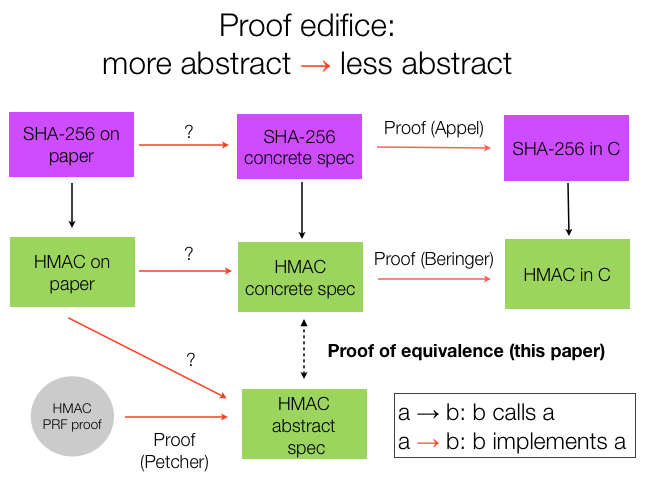
\includegraphics[scale=0.35]{Proof_edifice}
	\caption{Mind the gap (the dotted arrow).}
\end{figure}	

\subsection{Formal verification in Coq}

Coq is a proof assistant.

Coq has two internal languages, Gallina and the tactic language. Gallina is a purely functional language similar to OCaml. The tactic language is used for doing proofs and defining new proof strategies.

As used here, formal verification of a piece of code means proving that this implementation fulfills some kind of high-level specification. The code will usually be written in a low-level language such as C and may contain optimizations and other tricks. The specification, or "spec," will usually be written in a high-level language such as OCaml or Gallina and is typically more mathematical and abstract.

For example, TODO sorting algorithm

TODO: insert diagram of what formal verification means

Coq has been used to

\subsection{The Merkle-Damgard construction}
% TODO add accent on Damgard
Say we have a strong cryptographic compression function TODO define. It has certain guarantees. However, it only operates on an input of a fixed length.

The Merkle-Damgard construction (referred to as "M-D" from now on) is a way to extend this function to inputs of any length by iterating the compression function on identically-sized, adjacent blocks of the input. It has been proven to uphold the desirable properties of C such as

\begin{figure}[h!]
	\centering
	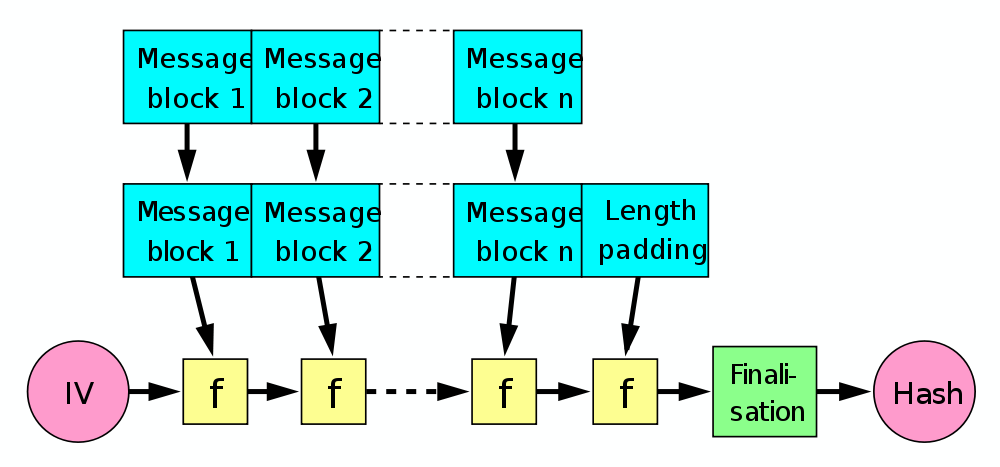
\includegraphics[scale=0.24]{Merkle-Damgard}
	\caption{The M-D construction.}
\end{figure}

SHA-256 is an example of an application of M-D.

Picture of crypto system 

\subsection{SHA-256}

SHA-256 is a cryptographic hash algorithm used for TODO. Mention OpenSSL.

It operates on a message of any length by breaking the message into 512-bit blocks. TODO (is this right?) It outputs a 256-bit digest. 

Like all such hash functions, it comes with guarantees of TODO (collision resistance...)

Inner hash function

PRF

\subsection{HMAC}

A message authentication code is used to

HMAC uses SHA-256. 

HMAC's code is: (SHORT CODE HERE)

Mention OpenSSL.

\begin{figure}[h!]
	\centering
	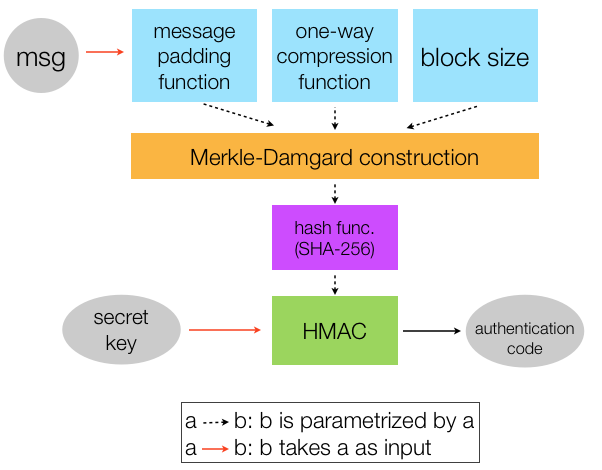
\includegraphics[scale=0.4]{Cryptosystem}
	\caption{The entire system. It is slightly more correct to think of a "black box" HMAC taking message and key as input, and outputting the authentication code.}
\end{figure}

\subsection{Prior work}

Verification of SHA-256.

\section{The proof of equivalence}

\subsection{The concrete HMAC spec}

Operates on bytes. Runnable code. Calls the spec of SHA-256.

\subsection{The abstract HMAC spec}

It includes the GNMAC/\verb|GHMAC_2K| structures. It leaves the hash function, two padding functions, and the hash function's initialization vector abstract.

Parameters:

\subsection{Instantiating the abstract specification}

We wrap the concrete functions in byteToBit and/or \verb|intlist_to_Zlist| conversion functions. 

Code:

\subsection{Proof outline}

Equivalence of specs means 

\begin{figure}[h!]
	\centering
	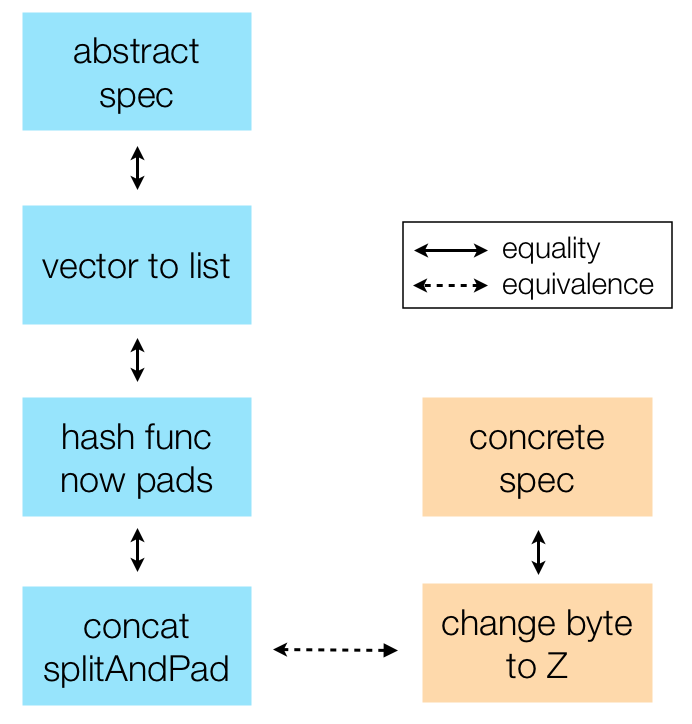
\includegraphics[scale=0.56]{Equivalence_proof_chain}
	\caption{Stages of the equivalence/equality proofs.}
\end{figure}

The main differences between the specs are that (make a table?)
\begin{enumerate} 
\item the abstract spec operates on bits, whereas the concrete spec operates on bytes
\item the abstract spec uses the dependent type \verb|Bvector n|, which is a bit list of length $n$, whereas the concrete spec uses byte lists and int lists
\item the abstract spec pads its input twice in an ad-hoc manner, whereas the concrete spec uses the SHA-256 padding function consistently
\item the SHA-256 concrete spec uses the Z type, whereas the HMAC concrete type uses the byte type, which is Z constrained to be in $[0, 255]$.
\end{enumerate}

\subsection{Proof techniques}

We reasoned about the bytes/bits proof via the following two frameworks.

\begin{itemize}
\item (Round-trip and conversion properties. Galois connections or other algebraic structure?)
\item Wrapped function equivalence on application. Interestingly, we have equivalence when a "round-trip" of composing the two transportation functions results in the identity function.
\item Wrapped function equivalence on repeated application: depends on the previous one, and is completed by induction on the number of applications. This corresponds to the SHA-256 operation of hashing blocks.
\end{itemize}

The following techniques may be useful in future equivalence proofs.

\begin{itemize}
\item Many theorems are true for lists of any length (e.g. some involving map and zip). We found it difficult to do dependent type induction. Instead, we found it easy to prove theorems by induction on a Blist, implying that the list may be any length, then specialize it to \verb|Bvector n|, a Blist of length $n$. 
\item Likewise, we found it easier to prove theorems about lists of any length (or a certain length given by an assumption), then prove that the functions involved preserve the length. This is equivalent to working with \verb|Bvector n|.
\item When dealing with lists whose lengths must be a multiple of a block size (e.g. 512 bits or 64 bytes), we found it useful to define an inductive proposition \verb|InWords n l| that would allow one to do proofs by inducting in the block size, cons'ing elements to the front. We then proved this equivalent to the computational version (using the length function).
\item Likewise, we found it useful to define two things: a function to compute conversions between byte lists and bit lists, and an inductive proposition stating that the lists correspond in this way.
\item When it comes to theorems that involve tricky math, we exploited the fact that range of a byte is $[0, 255]$ and proved them by brute force instead. The same technique also works in reverse. Proving something true for $8$ booleans is as simple as checking that the statement is true for each of the $256$ cases.
\end{itemize}

\subsection{Problems encountered}

\begin{itemize}
\item We found it difficult to work with dependent types, induction, and John Major equality.
\item We encountered problems converting between many machine representations: byte/Z, byte/bit, int/Z, and even little-endian vs. big-endian.
\item We did not find much prior work on this sort of equivalence proof, except for related functions in Coq.Strings.Ascii.
\end{itemize}

\section{The proof of HMAC's safety}

\subsection{The 1996 (?) Bellare proof}

Let $f$ be the compression function and $f^*$ the iteration of $f$.

Given the assumption that $f$ is a pseudo-random function (PRF), that implies that $f^*$ is computationally almost universal ($cAU$). $cAU$ is a slightly weaker property than collision-resistant.

% (\verb|goo.gl/wK8OXg|)
\begin{figure}[h!]
	\centering
	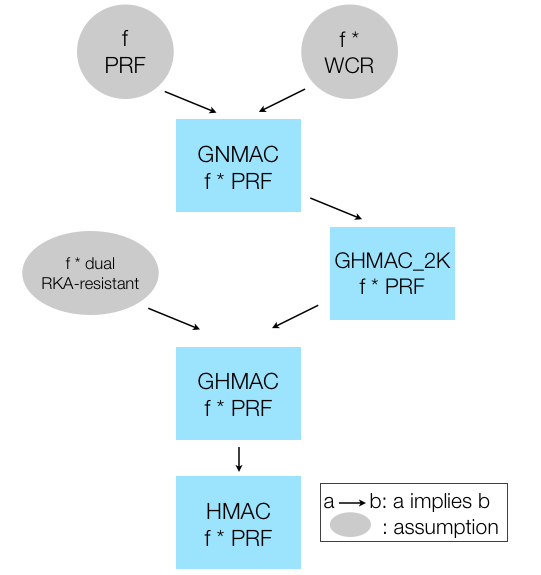
\includegraphics[scale=0.4]{HMAC_proof}
	\caption{The structure of the 1996 (? TODO) Bellare HMAC proof.}
\end{figure}

The $f^* cAU$ property is used to prove that generalized NMAC (GNMAC) using $f^*$ is a PRF. The GNMAC property is used to prove that generalized HMAC with two keys (\verb|GHMAC_2k|) using $f^*$ is a PRF.

Using that fact and the assumption that $f^*$ is RkA-resistant (?), we prove that GHMAC (single-keyed) using $f^*$ is a PRF. This, plus the fact that the padding function for $f$ is one-to-one, leads finally to the proof that HMAC using $f^*$ is a PRF.



\subsection{Formalization in Coq}

See Adam Petcher's paper on MCF. Random oracles, monadic syntax.

\subsection{Transfer of properties}

In order for the the proof to hold, the following assumptions must be true:
\begin{itemize}
\item the padding function (which? TODO) is one-to-one
\item opad and ipad differ in at least one bit.
\item (anything else? TODO)
\end{itemize}

Examining the final spec, these are true. TODO

Thus, the property TODO transfers. (termination and well-definedness of C code? Adam's email?)

Interfaces that drop out of the proof are TODO, leaving an end-to-end proof of correctness.

\section{conclusion}

Contribution to cryptography: bridging the gap between concrete and abstract HMAC specs allows the desirable property of being a PRF to transfer to the OpenSSL implementation of HMAC. So it's "safe to use."

Contribution to reasoning about equivalence: many bytes/bits computational and inductive definitions. Lemmas for correspondence between them. 

Contribution to proof techniques: results of trying to use dependent types. Brute force. Inductive propositions for length, plus InBlocks correspondence with division, mod, and existence.

\subsection{Future work}

Dependent types, type-level programming in Coq.

Libraries could be written to aid reasoning about equivalence and lengths.

More crypto formalization! EasyCrypt, CertiCrypt, IMDEA. MCF

SHA PRF, of course

How to transmit HMAC key? Need RSA. Work being done at Princeton.


\begin{acknowledgments}

Andrew Appel, Lennart Beringer, Adam Petcher, and Qinxiang Cao.

\end{acknowledgments}

\section{references}

"Verification of SHA-256," Appel (unpublished?)

"New Proofs for NMAC and HMAC: Security without Collision-Resistance," Bellare (1996)

"Keying Hash Functions for Message Authentication," Bellare (2004)

"MCF," Petcher (unpublished?)

"Merkle-Damgard in EasyCrypt," IMDEA

"Certified Programming with Dependent Types," Chlipala

"Software Foundations," Pierce et al.

Coq.Strings.Ascii

\section{appendix}

\subsection{The concrete HMAC spec}

\subsection{The abstract HMAC spec}

\subsection{Definitions}

\subsection{The equivalence proof}

\subsection{Selected theorems and proofs}

\end{document}